
\chapter{Implementation}

\section{Operation}
Operations are used to decribe changements made in a document. For this purpose they must contain the information: \emph{what} has been changed and \emph{where} it has been changed.

In case of simple text editing only two operations are required. An insert operation (e.g. \texttt{Ins(1,'hello')}) which will insert the string 'hello' at position 1 and an delete operation (e.g. \texttt{Del(10, 'world')}) which will delete the string 'world' at position 10.

\begin{figure}[H]
\centering
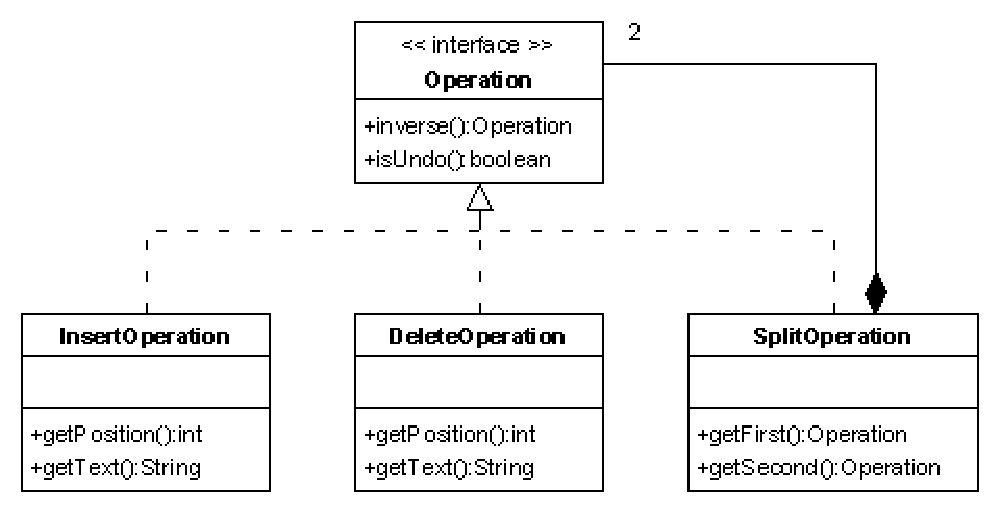
\includegraphics[height=5.74cm,width=11.59cm]{../../images/algo-impl/operation_classdiagram.eps}
\caption{Operation Hierarchy}
\label{Operation Hierarchy}
\end{figure}

\label{Split_Operation}
As depicted in figure \ref{Operation Hierarchy} there exists a third operation besides the \texttt{InsertOperation} and \texttt{DeleteOperation}. The so-called \texttt{SplitOperation} is a helper object used to encapsulate two operations (usually two delete operations). This special operation is required when transforming an insert operation which occurs in the range of a delete operation. For more details about transformation functions see \ref{GOTO Transformation Functions}, especially the spitting scenario described in \emph{Case 8} in \ref{Delete_Insert}.

\section{Request}
A request is used to distribute changes of a document over the network. It contains all important information such as an operation (what has changed and at which position), a timestamp (document state on which the operation is based) and the site id of the generating site. (see figure \ref{Request Class Diagram})

\begin{figure}[H]
\centering
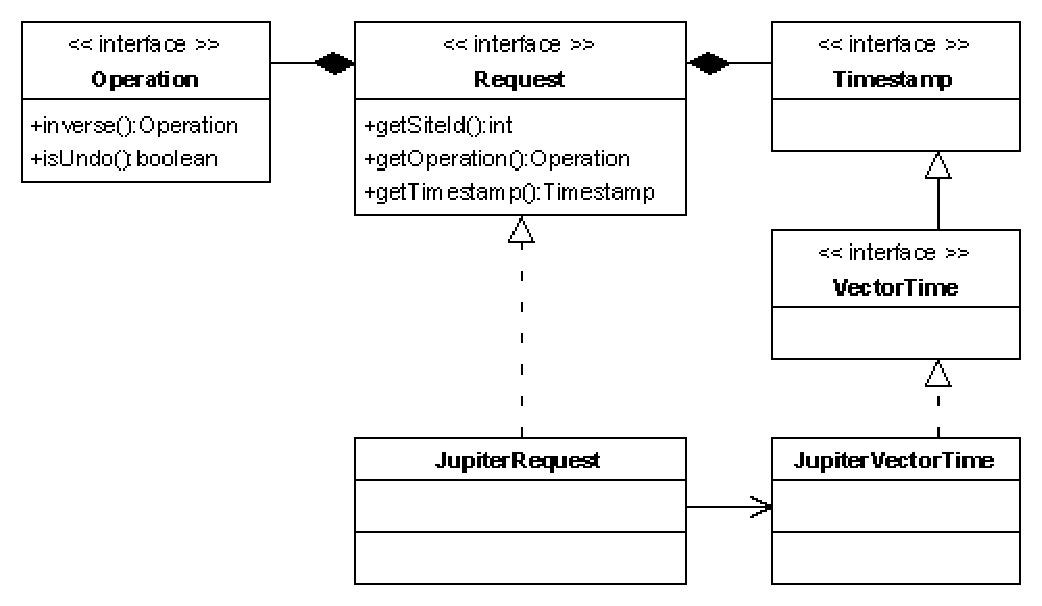
\includegraphics[height=6.87cm,width=12.09cm]{../../images/algo-impl/request_classdiagram.eps}
\caption{Request Class Diagram}
\label{Request Class Diagram}
\end{figure}

How a request will be sent to a server or another client is not part of this chapter and depends on the network technology (see \emph{Report Evaluation Network}) used.


\section{Algorithm}
\begin{figure}[H]
\centering
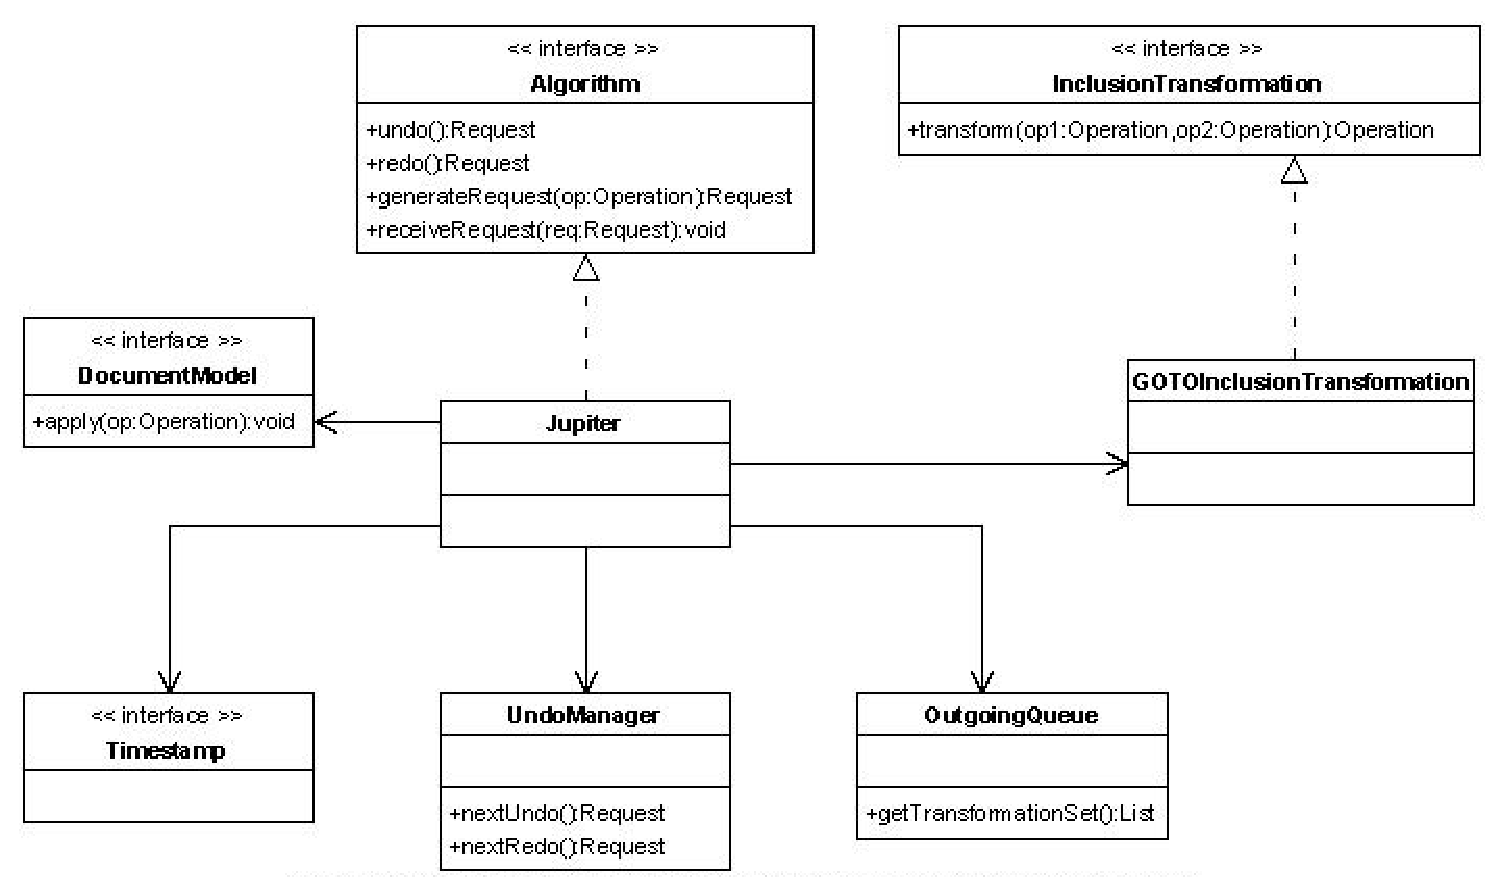
\includegraphics[height=8.74cm,width=14.95cm]{../../images/algo-impl/algorithm_diagram.eps}
\caption{Algorithm architecture}
\label{Algorithm architecture}
\end{figure}

The algorithm component centers around the \texttt{Jupiter} class, which is an implementation of the \texttt{Algorithm} interface. \texttt{Jupiter} processes all requests with the collaboration of the GOTOInclusionTransformation. All transformed operations are applied to the DocumentModel instance. The \texttt{Timestamp} class represents the current version of the document. In the case of the \emph{Jupiter} algorithm, the timestamp is a vector time. The vector time represents the current location in the 2-dimensional state space of the \emph{Jupiter} algorithm. The \texttt{UndoManager} class is used for undo/redo functionality and is further described in \ref{undo_redo}. The \texttt{OutgoingQueue} stores all requests that remain to be acknowledged by the server. A request is acknowledged if the state vector of an incoming request indicates that the server has processed the request.

The idea behind the \texttt{Algorithm} interface is to have the flexibility to switch the algorithm implementation without affecting the rest of the system.

\section{Synchronized Blocking Queue}
Throughout the implementation of the client and the server, synchronized blocking queues (\texttt{SynchroniziedQueue}) are used to decouple senders and receivers. It provides snychronized insertion for senders. Receivers will block when trying to retrieve from an empty queue. If the queue is not empty, the first object from the queue is returned and removed from the queue. The queue is based on the first-in-first-out (FIFO) principle.


\section{Client}
\begin{figure}[H]
\centering
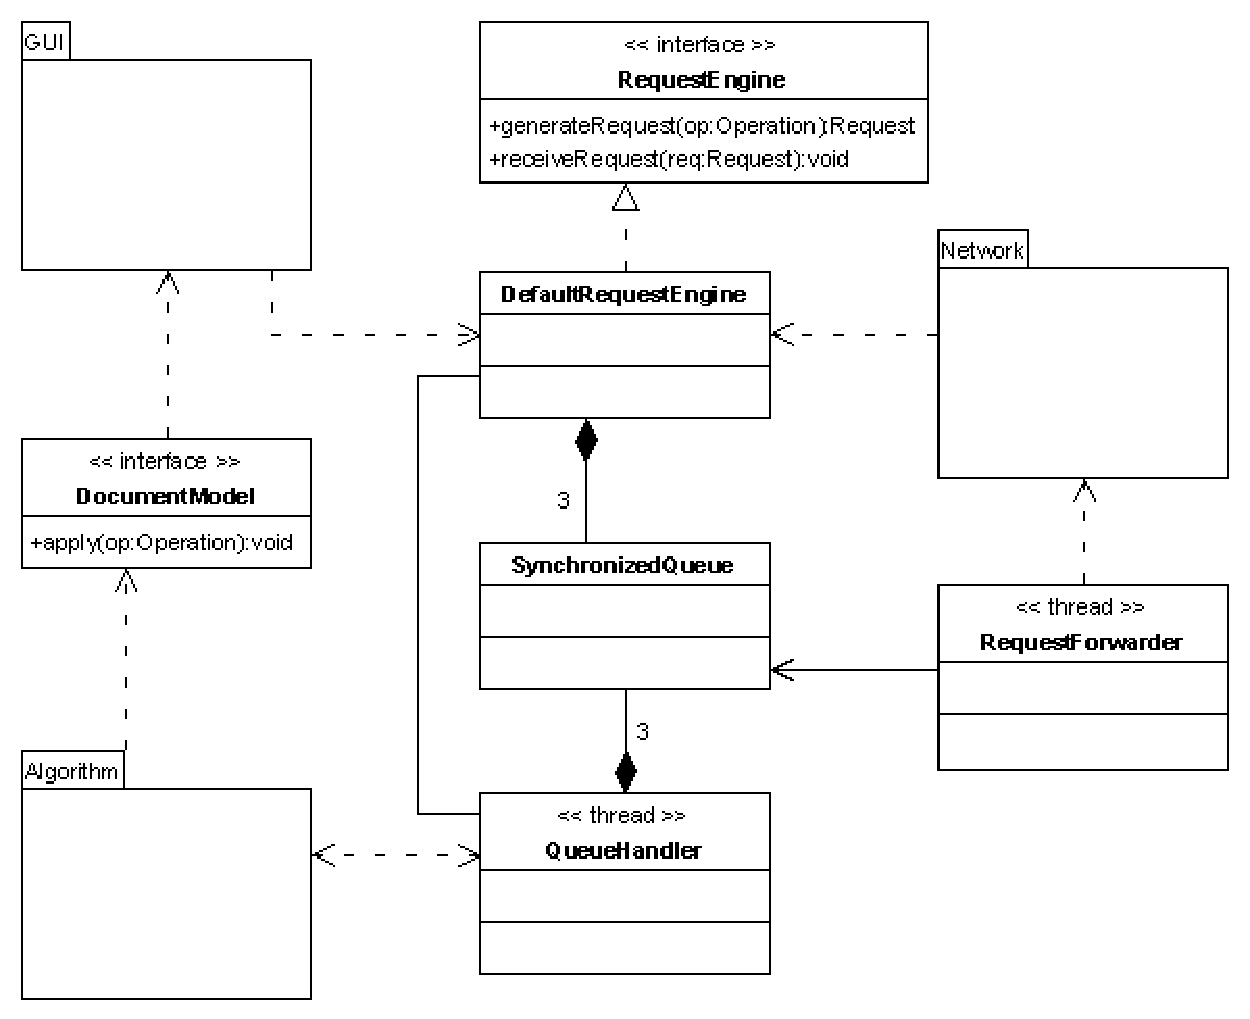
\includegraphics[height=13.04cm,width=15.46cm]{../../images/algo-impl/client_diagram.eps}
\caption{Client architecture}
\label{Client architecture}
\end{figure}

The client architecture centers around the \texttt{RequestEngine} class. The \texttt{RequestEngine} is a mediator between the GUI, network and algorithm components. It receives requests from the GUI and the network, respectively. All requests are passed to synchronized blocking queues, one for local requests and one for remote requests. The requests are read out from the queues by the \texttt{QueueHandler} class. This thread waits on the queues until a request is received. Each request is then handed to the algorithm package for processing. Processing involves transforming the operation and applying it to the document model. 

Locally generated requests are returned from the algorithm package to the \texttt{QueueHandler} which in turn passes it to another synchronized blocking queue, namely the outgoing queue. From there, all outgoing requests are forwarded to the network package by the \texttt{RequestForwarder} class. 

The idea behind the \texttt{Algorithm, GUI and Network} packages is to have the flexibility to switch an implementation without affecting the rest of the system.

\subsection{Workflow}
The workflow of the \emph{Jupiter} client is depicted in the following figure.
\begin{figure}[H]
\centering
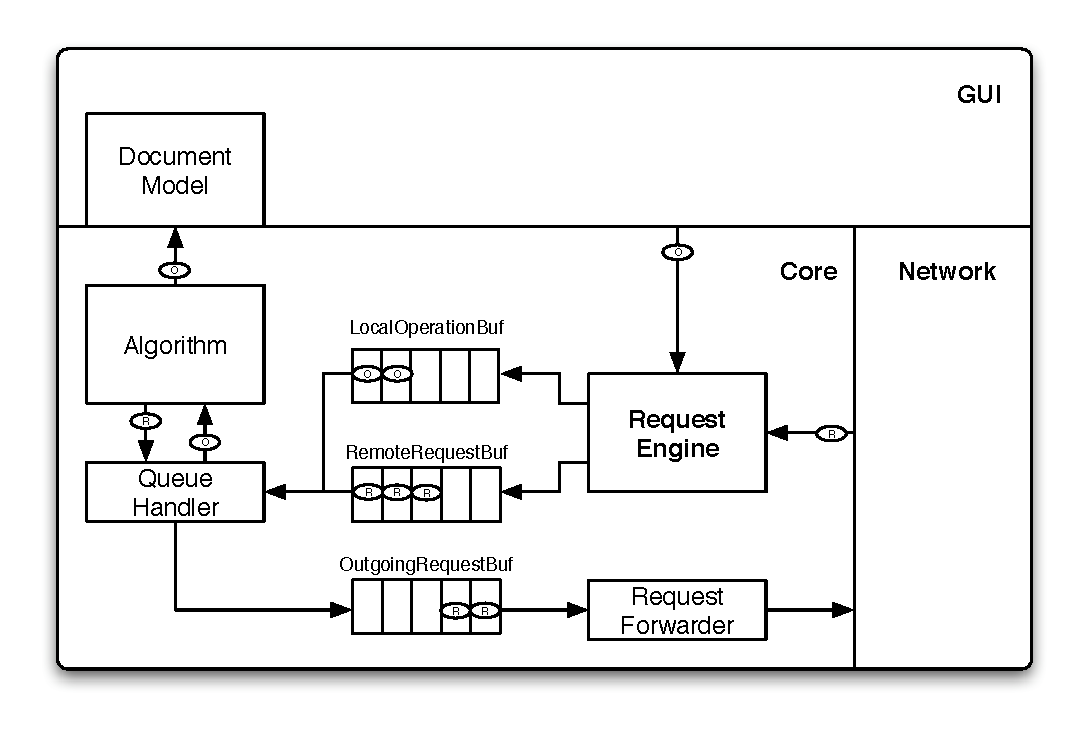
\includegraphics[height=9.5cm,width=14.3cm]{../../images/algo-impl/workflow_client.eps}
\caption{Client workflow.}
\label{Client workflow.}
\end{figure}

\subsection{Sequence diagram: Generate local operation}
\begin{figure}[H]
\centering
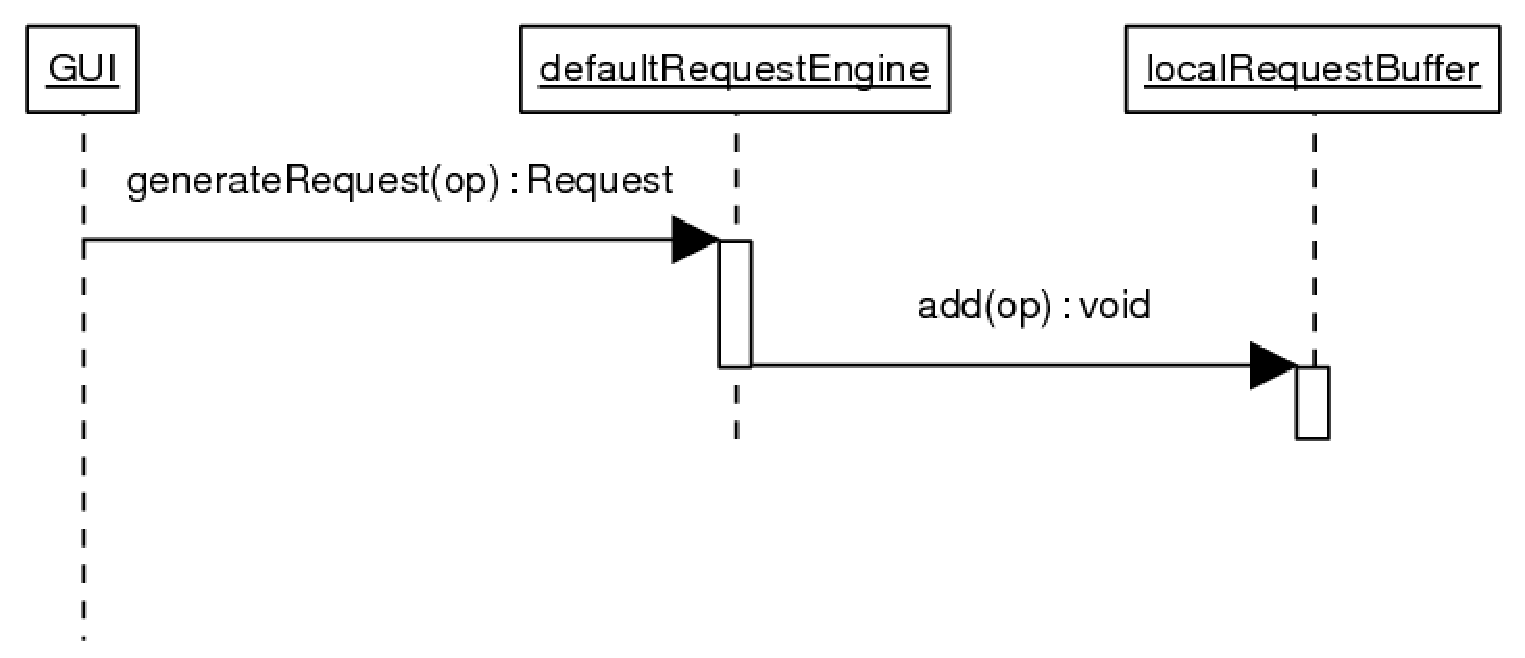
\includegraphics[height=4.23cm,width=10.09cm]{../../images/algo-impl/client_generate_request.eps}
\caption{From GUI to local operation buffer.}
\label{From GUI to local operation buffer.}
\end{figure}

\begin{figure}[H]
\centering
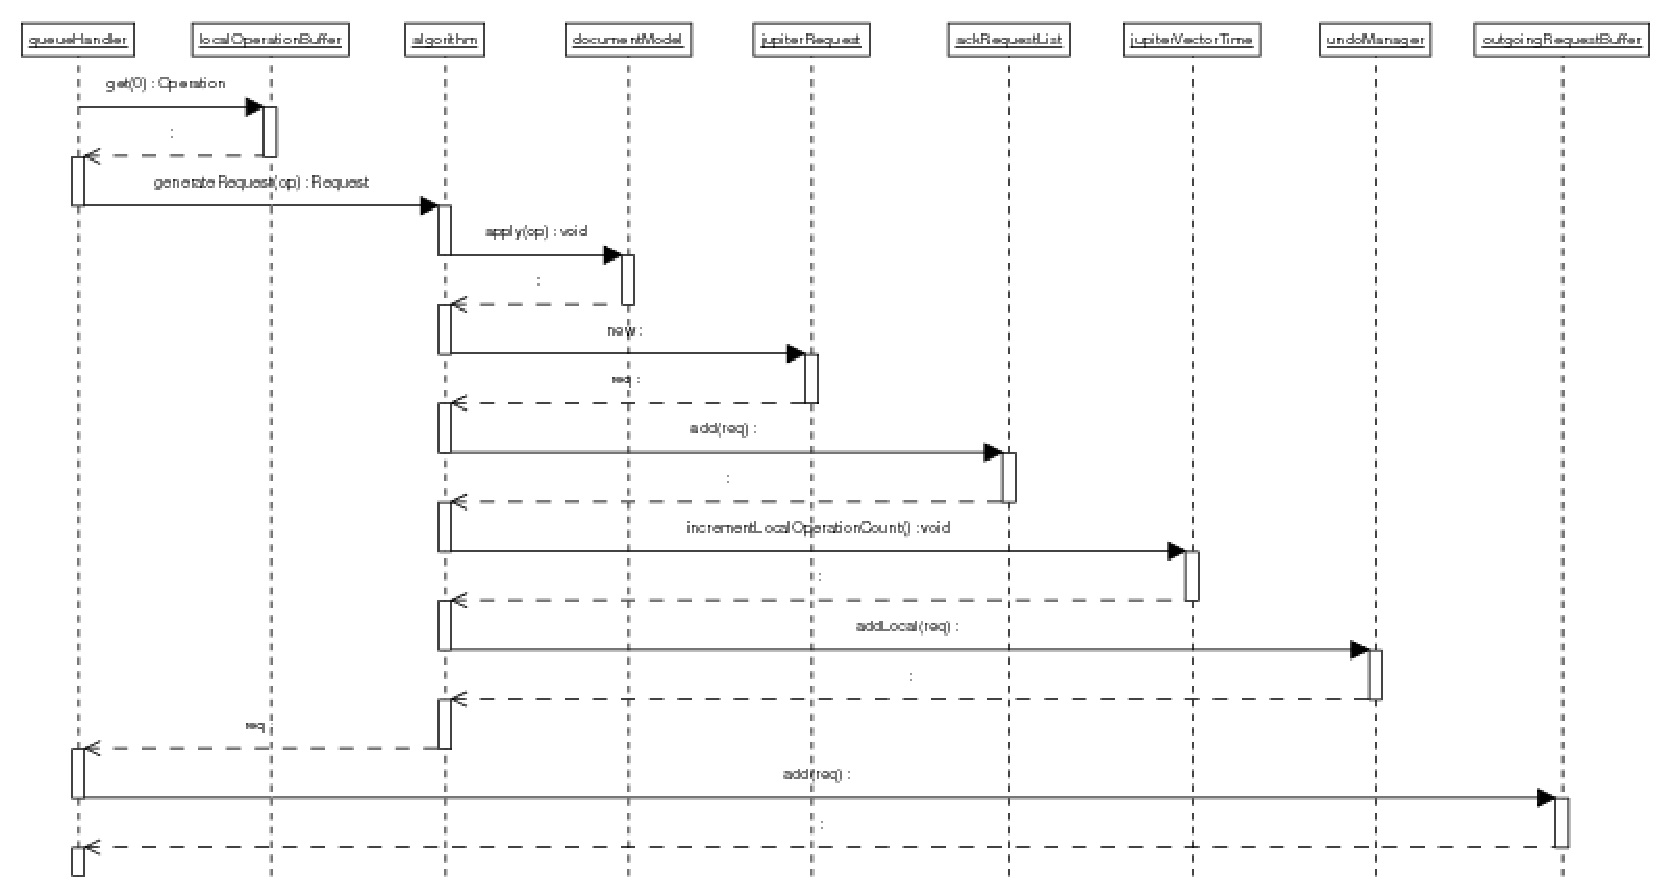
\includegraphics[height=7.3cm,width=13.86cm]{../../images/algo-impl/queue_handler.eps}
\caption{The queue handler processes the operation.}
\label{The queue handler processes the operation.}
\end{figure}

\begin{figure}[H]
\centering
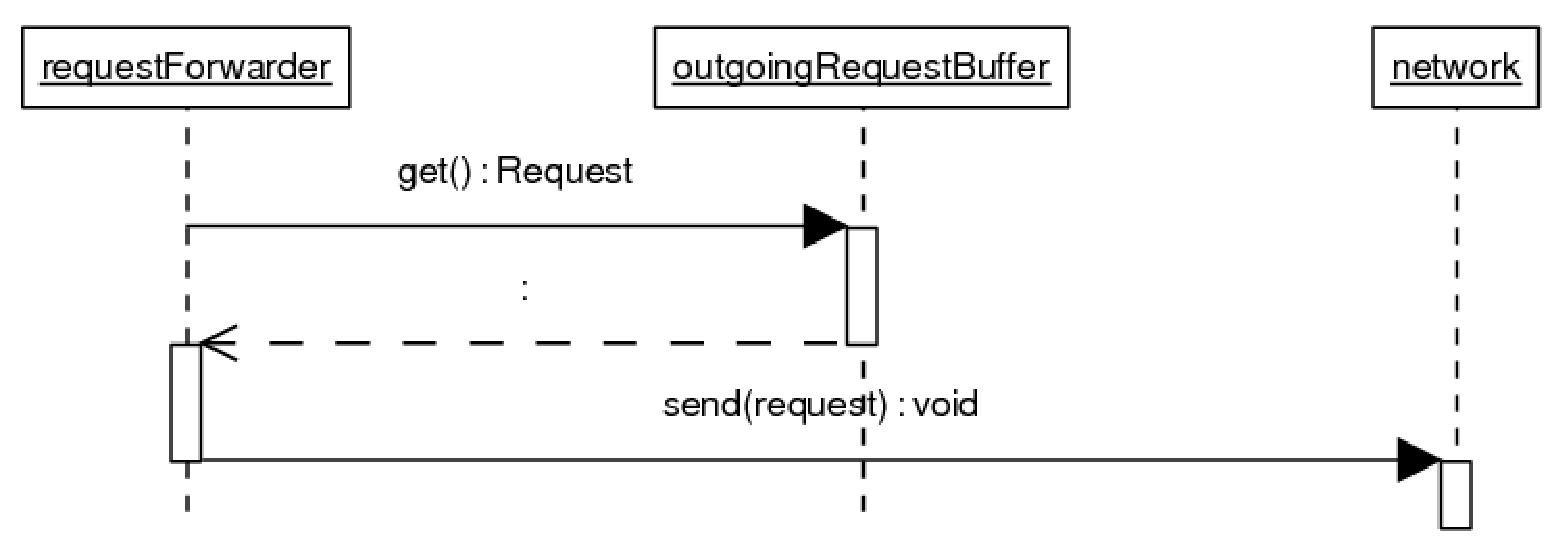
\includegraphics[height=3.42cm,width=10.09cm]{../../images/algo-impl/requestForwarder.eps}
\caption{The request forwarder hands the request over to the network.}
\label{The request forwarder hands the request over to the network.}
\end{figure}

\subsection{Sequence diagram: Receive a remote request}
\begin{figure}[H]
\centering
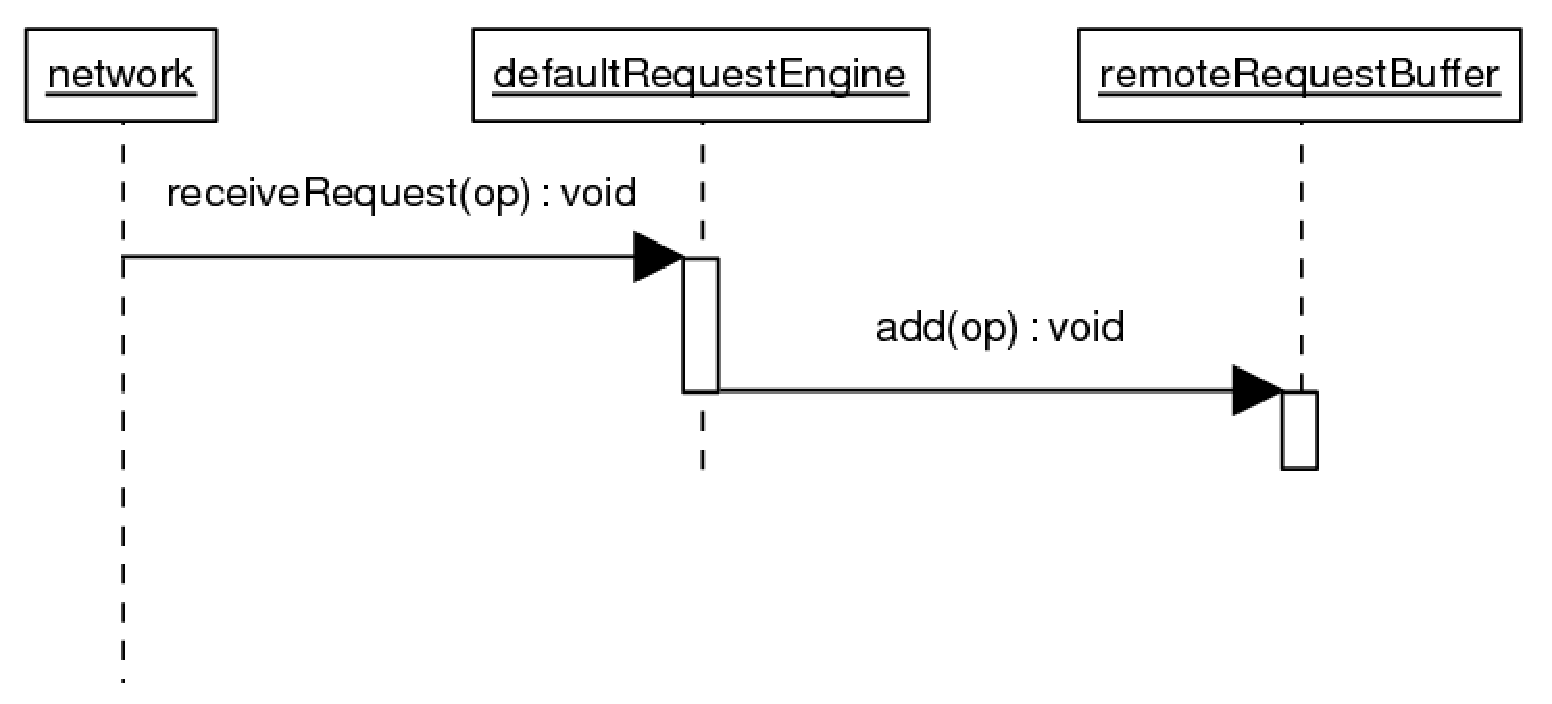
\includegraphics[height=4.48cm,width=10.09cm]{../../images/algo-impl/client_receive_request.eps}
\caption{From network to remote request buffer.}
\label{From network to remote request buffer.}
\end{figure}

\begin{figure}[H]
\centering
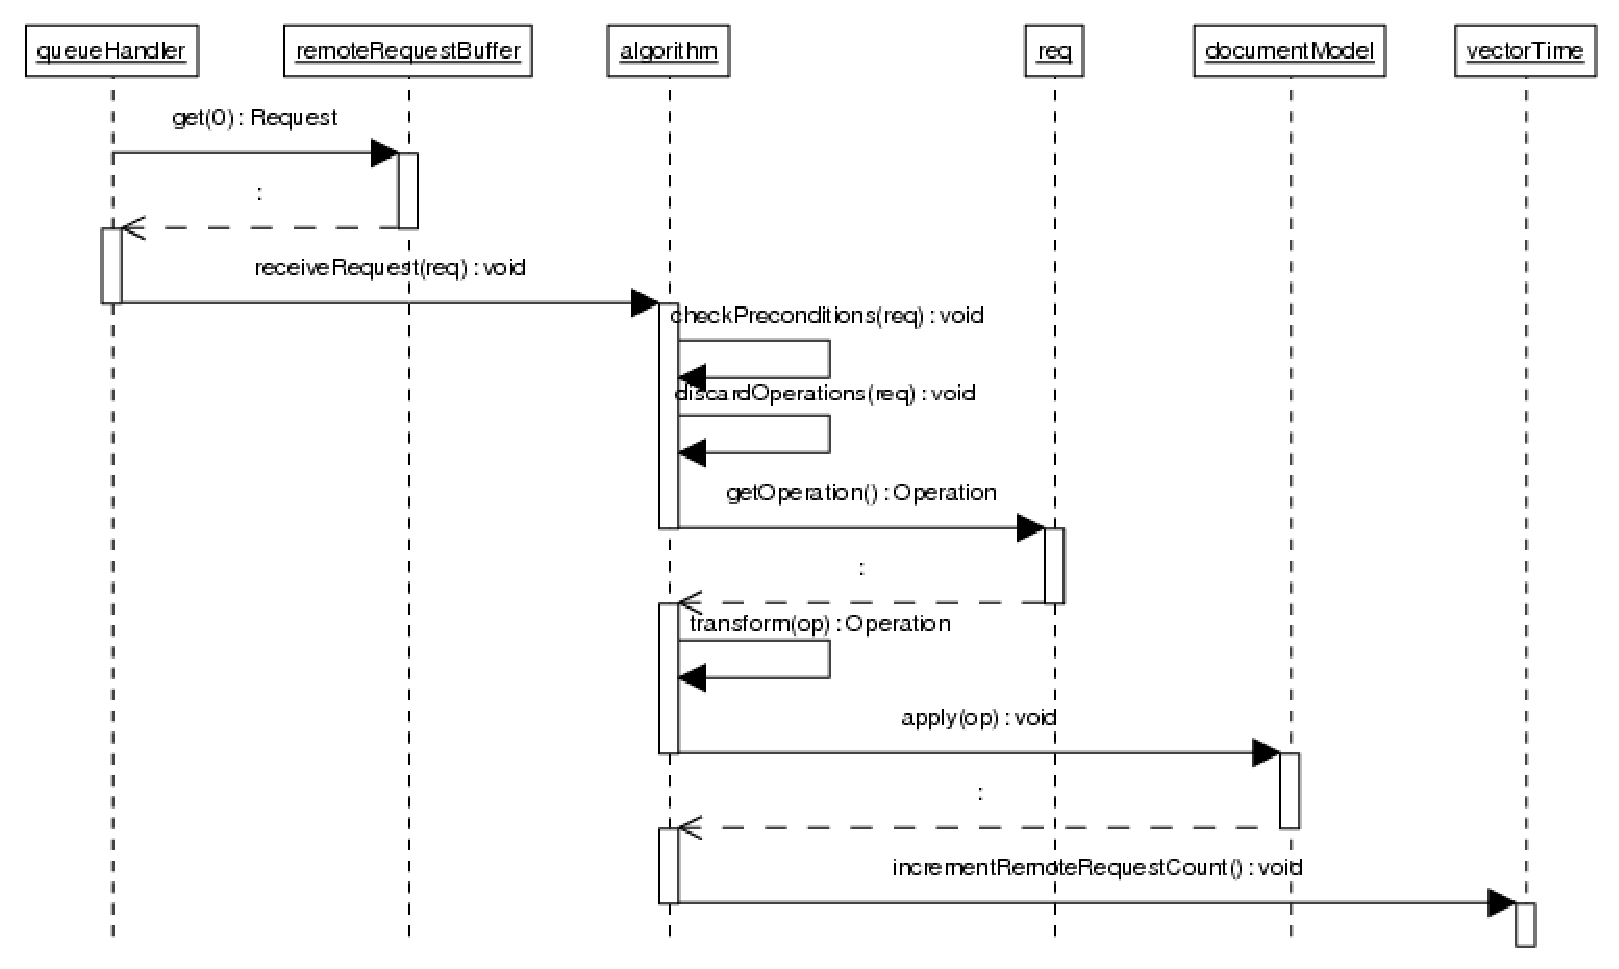
\includegraphics[height=8.71cm,width=14.76cm]{../../images/algo-impl/queuehandler_receive_request.eps}
\caption{The queue handler processes the request.}
\label{The queue handler processes the request.}
\end{figure}


\section{Server}
\begin{figure}[H]
\centering
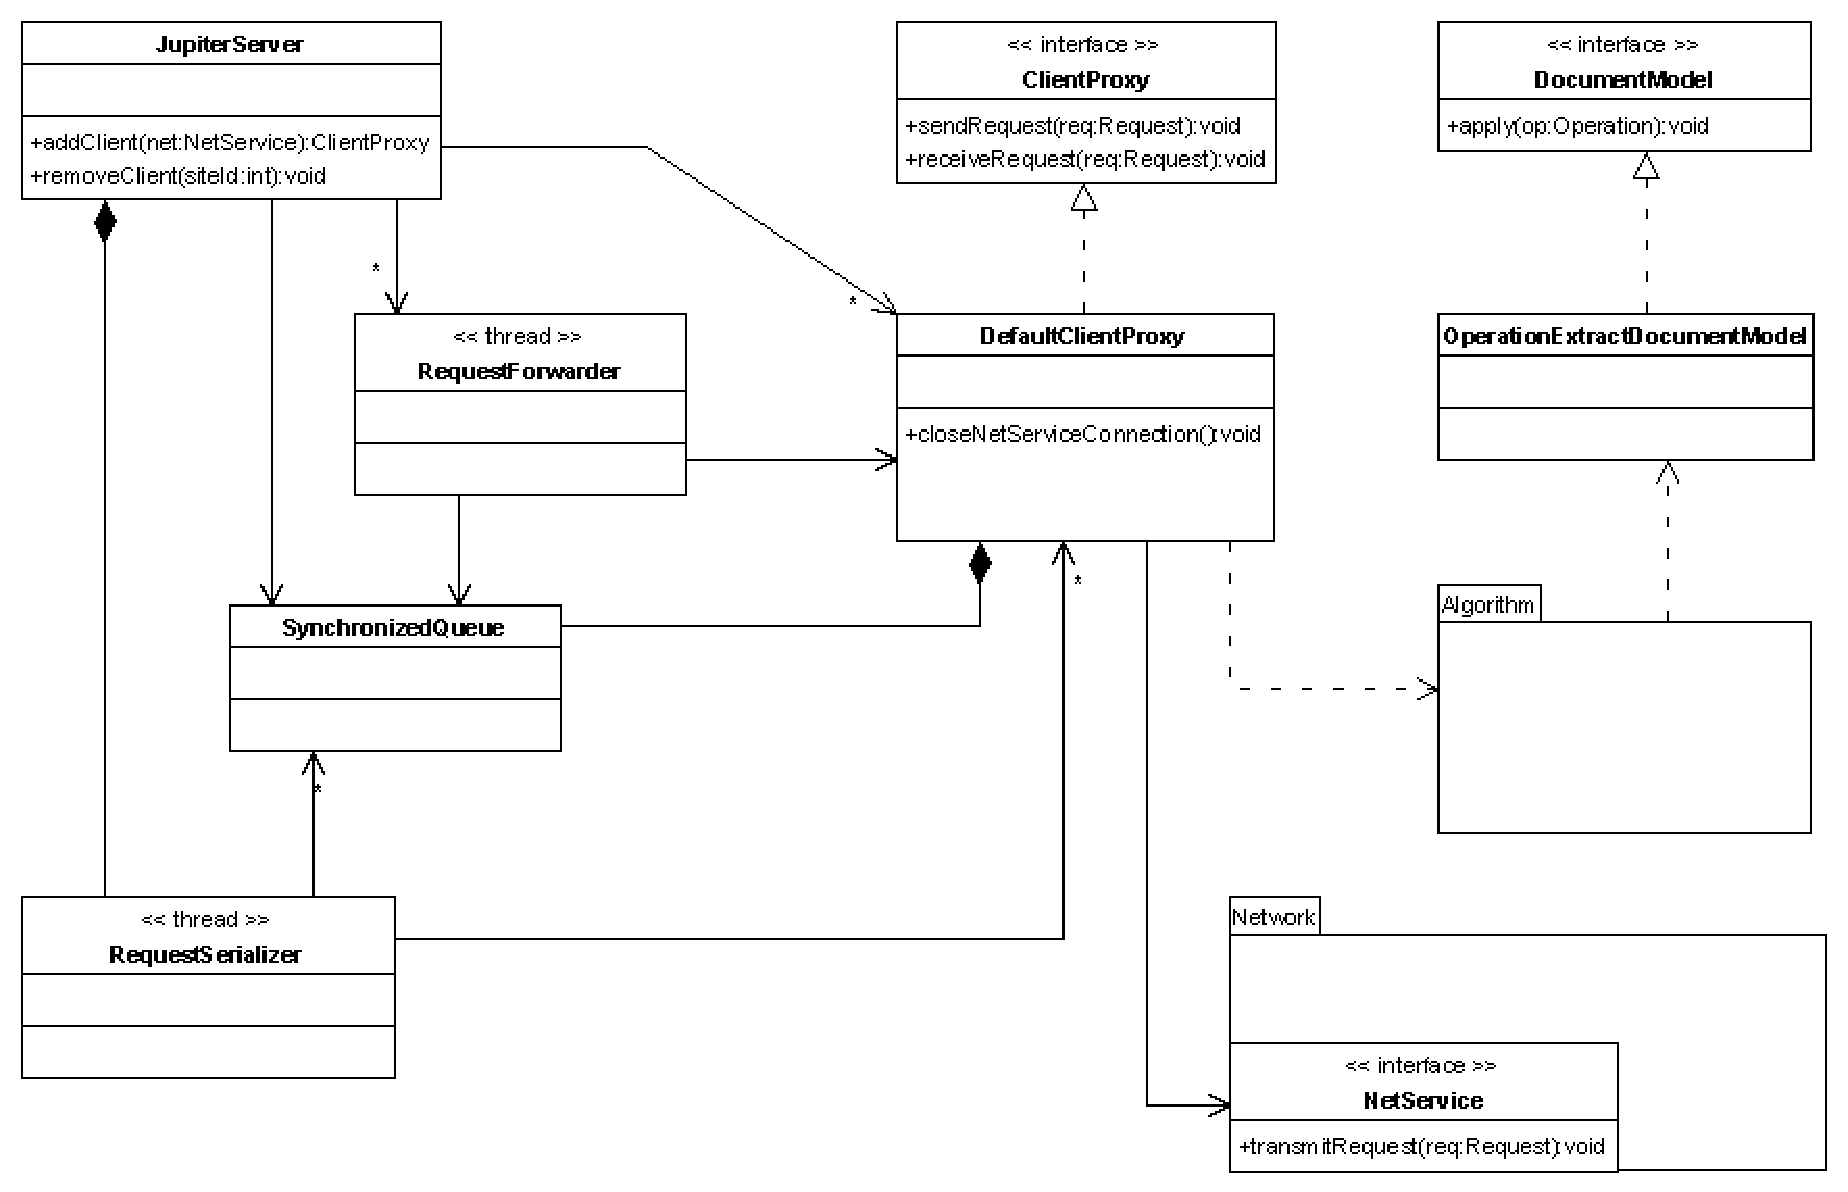
\includegraphics[height=9.8cm,width=15.36cm]{../../images/algo-impl/server_diagram.eps}
\caption{Server architecture}
\label{Server architecture}
\end{figure}

The \emph{Jupiter} server component is the turntable in a multi-user collaborative editing session. It achieves n-way communication by use of the 2-way synchronization protocol of \emph{Jupiter} between each client and its corresponding \texttt{ClientProxy} on the server side (instances of class \texttt{ClientProxy}). The \emph{Jupiter} server component can be started and organized by creating a new instance of class \texttt{JupiterServer}. It allows to add and remove client proxies.

\subsection{Adding a client}
When a new client is added to the server, a new \texttt{ClientProxy} is created. It is passed references to instances of the following types: \texttt{NetService}, \texttt{Algorithm} (\texttt{Jupiter}), \texttt{SynchronizedQueue}. The \texttt{NetService} class is used to forward outgoing requests to the network layer. The algorithm is responsible for the operational transformation. Since no real document model is used at the server side, a special implementation of the \texttt{DocumentModel} interface, OperationExtractDocumentModel, lets the algorithm extract the latest applied operation.

Afterwards, the \texttt{ClientProxy} instance is added to the \texttt{RequestSerializer}. Finally, a RequestForwarder for this \texttt{ClientProxy} is created. It is responsible for forwarding all requests that were issued by other clients and are to be sent to the \texttt{ClientProxy}'s client, namely the client itself. The \texttt{RequestForwarder} reads requests from the \texttt{SynchronizedQueue} and passes them to the \texttt{ClientProxy} by invoking \texttt{sendRequest(request)}.

\subsection{Removing a client}
When a client proxy is to be removed, firstly its connection to the net service is closed. Then the \texttt{RequestForwarder}, belonging to the client proxy, is shut down. Finally, the client proxy is removed from the \texttt{RequestSerializer}. The removal from the \texttt{RequestSerializer} is more complicated. At the time of removal, there may still be a couple of requests which have been issued by the client to be removed. Therefore, the client proxy may not be removed until all these requests have been processed, i.e. transformed and sent to all other clients. This is done by remembering the number of requests in the request queue, say $r$. After $r$ requests have been processed from that moment on, the client proxy can savely be released. This mechanism is achieved by a helper class named \texttt{Counter}.

\subsection{Workflow}
The workflow of the \emph{Jupiter} server is depicted in the following figure.
\begin{figure}[H]
\centering
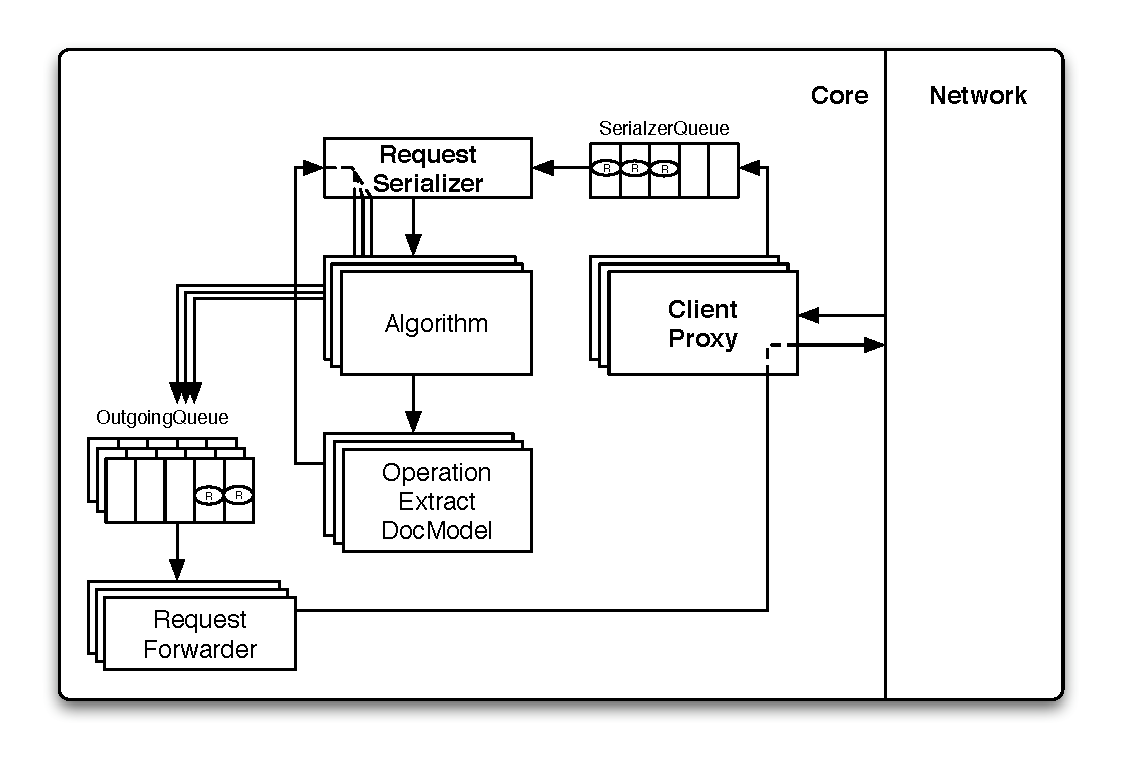
\includegraphics[height=9.64cm,width=14.3cm]{../../images/algo-impl/workflow_server.eps}
\caption{Server workflow.}
\label{Server workflow.}
\end{figure}

\subsection{Receiving and sending a request}
The received request is passed from the network layer to the corresponding \texttt{ClientProxy} instance. The {ClientProxy} itself only forwards the request to the {SynchronizedQueue}, namely request queue. Actually all {ClientProxy}'s forward their requests to the same synchronized queue. By that, a global serialization is achieved. From the request queue, the request is read out by the \texttt{RequestSerializer} thread. The request is then passed to its corresponding client proxy for transformation. Afterwards, the transformed request is distributed to all other clients. This is done by first calling \texttt{generateRequest(operation)} on each \texttt{ClientProxy}'s algorithm and then adding the returned request to the outgoing queue of the \texttt{ClientProxy}. From there, the \texttt{RequestForwarder} will read out the request and pass it to the \texttt{ClientProxy} which in turn forwards it to the net service. Finally, the net service transmits the request to the client.

\section{Undo/Redo}
\label{undo_redo}
For the undo implementation, we worked closely with the paper "Reducing the Problems of Group Undo" from Ressel et al., adapting the \emph{adOPTed} undo for the \emph{Jupiter} algorithm. The implementation of undo functionality has started but has not finished by the time. The undo works in simple cases both for characterwise and stringwise operations. But it fails in more complex scenarios (cf. classes $JupiterCharUndoTest.java$ and $JupiterStringUndoTest.java$, respectively. At first, we assumed that we could implement the undo with some auxiliary data structures and would not have to build the whole state space. In fact, it worked for example 1 on page \pageref{example1} as well as for example 3 (see page \pageref{example3}, also known as the 'del-del-undo-puzzle') described in the undo section, but it finally failed at the 'order puzzle' (see example 2 on page \pageref{example2}). The 'order puzzle' showed us that the auxiliary data structures would not be sufficient for more complex undo scenarios and that we would need to implement the whole state space as is the case in the \emph{adOPTed} algorithm and undo, respectively. Therefore we will not further describe the undo implementation we have done so far as much of it will become unusable as soon as we implement the state space. Building the state space means keeping track of every operation and calculating all possible transformation paths. We also have to bear in mind that the state space cannot grow endlessly. Therefore we need to find a way to garbage collect it. This feature is also left open as future work.

Nevertheless, two issues will remain. Firstly, each operation has a method \texttt{isUndo()} to detect undo operations and to treat them separately. Secondly, the \texttt{UndoManager} class is used to manage undo and redo requests.

\section{Tests}
Testing the algorithm implementation was considered a very high priority. Without a correctly working algorithm, it will be difficult or even impossible to create a collaborative text-editor. Because of the significance of this algorithm we invested a lot of time to test it.

\subsection{Testframework}
In the literature about operational transformation, so called puzzles are omnipresent. These puzzles are exact specification of the order of events, like the generation of a request or the reception of a request. We were soon convinced that in order to test our algorithm it would be possible to have a testframework that accepts such a puzzle (called scenario) as input and replays the sequence of events on a set of algorithms. To find out more about this testframework, see the document emph{Report Implementation Testframework}.

\subsection{Test Cases}
We gathered many test cases form publications about operational transformation algorithms. The puzzles presented in these papers often represent particularly tricky issues that other algorithms failed to resolve. Here is a list of test cases that were taken from papers:

\begin{itemize}
 \item Figures 3, 4 and 5 in \cite{imine03b}
 \item "C2 puzzle P1" and "C2 puzzle P2" (figures 3 and 5, respectively) in \cite{imine04}
 \item "A scenario of divergence and ERV" and  "A divergence and ERV scenario of IMOR" (figures 1 and 12, respectively) in \cite{li04}
 \item figure 5 in \cite{suleiman98}
 \item the "dOPT puzzle" (figure 2) in \cite{sun98b} 
\end{itemize}

Our algorithm is capable of solving these complex puzzles. This is a step in the right direction, but that alone is not enough. So we devised additional test cases that cover trivial as well as complex scenarios.

\subsection{JUnit Tests}
It is one of our goals to have a good test coverage with \emph{JUnit} tests.
